\documentclass[a4paper, fontsize=12pt, ngerman, oneside, openright]{scrreprt}

% Rendering packages
\usepackage{amsmath}
\usepackage{amssymb}
%\usepackage[draft]{graphicx}
\usepackage{graphicx}
\usepackage{wrapfig}
\usepackage{svg}
\usepackage{subcaption}
\usepackage{placeins}
\usepackage{xcolor}      % use if color is used in text
\usepackage{eurosym}


% Page dimensions
\usepackage[inner=3.5cm,outer=2.5cm,top=3.7cm,bottom=3.5cm]{geometry} 
\usepackage{parskip}
\usepackage[onehalfspacing]{setspace}

% Font styling
\usepackage[english]{babel}
\usepackage[utf8]{inputenc}
\usepackage[T1]{fontenc}
\usepackage{lmodern}
\renewcommand\familydefault{\sfdefault}
\usepackage[11pt]{moresize}

% Tables
\usepackage{tabularx}
\usepackage{tabulary}
\usepackage{longtable, lscape}

% Headers
\usepackage{scrpage2}  % header and footer for KOMA-Script
\pagestyle{scrheadings}
\automark[section]{chapter}

% Zitate
\usepackage[backend=biber, 
			style=authoryear,
			isbn=false, 
			sorting=nyt,
			]{biblatex}
\usepackage[babel,german=quotes, english=british, threshold=3]{csquotes}
\bibliography{Bibliothek/Bibliothek}

\usepackage[hyperindex,breaklinks,colorlinks=true,linkcolor=black,urlcolor=blue,citecolor=black]{hyperref}

% Code Blöcke
\usepackage{listings}
%\usepackage{Header/listings-golang} % import this package after listings
\usepackage{syntax}



%\lstset{ % add your own preferences
%	frame=single,
%	captionpos=b,
%	mathescape=true,
%	basicstyle=\footnotesize\ttfamily,
%	keywordstyle=\color{black},
%	numbers=left,
%	numbersep=5pt,
%	showstringspaces=false, 
%	stringstyle=\color{blue},
%	tabsize=2,
%	language=Golang % this is it !
%}


%pdf insert
\usepackage{pdfpages}

%zusätzliche Trennungen
\hyphenation{Grund-ar-chi-tek-tur}
\hyphenation{MQTT-Kom-mu-ni-ka-tions-mo-dell}
\hyphenation{Master-Master-Replikation}
\hyphenation{Pub-lish-er}
\hyphenation{Pub-lish-ers}
\hyphenation{Sub-scriber}
\hyphenation{Sub-scribers}
\hyphenation{Pub-lish er/Sub-scriber}
\hyphenation{beo-bacht-bar}
\hyphenation{Score}
\hyphenation{Ac-knowl-edge-ment}
\hyphenation{Ac-knowl-edge-ments}

\usepackage{mathtools}
\DeclarePairedDelimiter\abs{\lvert}{\rvert}

\usepackage{acronym}



\begin{document}

% Titelseite einfügen.
\begin{titlepage}


\begin{center}
 		\includegraphics[scale=0.3]{Resources/Logo3}
\end{center}

\begin{center}
	\HUGE \textbf{Varroa}
	\large\\MQTT-Scenario-Testing-Tool\\ \ \\
	\small Masters Level Study Project, Prof. PhD. Siebert \\
	SS 2018 - WS 2018/2019
\end{center}

\begin{center}
R. Atherton, S. Baier, S. Giebl, G. Held, Y. Weber, T. Weiden
\end{center}

\end{titlepage}



% Counter zurücksetzen. Römische Ziffern einstellen.
\pagenumbering{Roman}
\setcounter{page}{1}

% Inhaltsverzeichnis generieren.
\tableofcontents

% Neue Seite. Counter zurücksetzen. Arabische Ziffern einstellen.
\pagenumbering{arabic}
\setcounter{page}{1}

% Kapitel einfügen.
\chapter{Vision}
The Name of our MQTT-Testing-Tool (Varroa) is inspired by the varroa mite, which is a species of mite that infects honey bee colonies.
This name has been chosen due to it working in a similar way but instead of infesting a hive, it tries to infest a broker.
The inspiration for this name came from the Broker \enquote{HiveMQ} and it's branding.
The basic use-case of Varroa is testing the resilience of Brokers by creating load.
Hereby load is defined by a number of MQTT-Clients sending different sequences of MQTT-messages to the Broker. 
Which sequences get carried out in which order is determined by a Scenario.
A Scenario is a concept which defines the temporal execution as well as the amount of actions across a MQTT-Network.
The motivation for the creation of this project was the lack of testability of MQTT-Systems without using large amounts of machines.
Therefore Varroa had to be a distributed System itself, to be able to test the Limits of a MQTT-Broker without using a machine for every client.

\chapter{Concepts}
To understand the workings of Varroa, we will have to take a look at the different parts that make up the system.
Furthermore we explain the basic concepts of MQTT.

\section{Varroa Distributed System Concepts}
A Varroa Distributed System orchestration of multiple Varroa instances consisting of one Commander and at least one Agent.
Varroa is organized as a distributed system, due to the impossibility of creating enough MQTT-clients on a single machine to overload a MQTT-broker, especially if the broker is also a distributed system.

\paragraph{Varroa Instance}
A Varroa instance is a running Varroa process in a single JVM, can be either Commander or Agent.

\paragraph{Commander}
The Commander is a part of the Varroa Distributed System, that parses the scenario, generates chunks and distributes them to the Agents.
Only one Commander exists in a Varroa distributed system.

\paragraph{Agent}
The Agent is part of the Varroa Distributed System.
It receives Chunks from the Commander and passes them to its MQTT-Agents.
A Varroa distributed system contains at least one Agent.

\paragraph{MQTT Agent}
MQTT Agents are components of an Agent.
Every MQTT Agent manages one MQTT client.

\paragraph{Chunk}
The scenario is split in Chunks by the Commander and then those Chunk are distributed to the agents.
%A Chunk is a Collection of Information, such as which commands are to be sent to the broker as well as how many clients should perform these commands.
%Another important information, contained in the Chunk is at which rate these commands are to be executed.

%A scenario is a XML-Document which defines a sequence of stages.

\section{Varroa Scenario Concepts}
The integral idea of Varroa is testing scenarios, which means simulating the behaviour of a large amount of MQTT clients.
It tests whether the broker can handle the associated load.
A scenario is an abstract representation of a real MQTT-Use-Case.
It defines the topology of all participating MQTT clients and brokers.

\paragraph{MQTT Client}
A MQTT client is used to execute the Commands to create load.
Those clients implement the MQTT protocol using the HiveMQ MQTT Client.

\paragraph{Client Group}
Client groups are part of the scenario.
They enable the user to define the behaviour and properties of a group of MQTT clients with a configurable size.
These MQTT clients are created by Varroa for the purpose of simulating the MQTT clients of a scenario.
The lifespan of the spawned MQTT clients does not exceed the lifespan of a scenario.

\paragraph{Command}
A command is an abstract representation of a work step that must be executed by a MQTT client.

\paragraph{Topic Group}
A Topic Group represents a number of topics that share a naming pattern.
This concept enables the user to model the interaction between Client Groups and a number of similar topics.

\section{General MQTT Concepts}
\paragraph{Broker}
The Broker serves as an intermediary between publishers and subscribers.
It takes over the routing of the exchanged MQTT messages and is the central control authority of a MQTT Network.
%TODO cite Georg
\paragraph{Client}
A client that implements the MQTT protocol. 
\paragraph{Topic}
Topics are strings separated by slashes that do not contain wild-cards.
Messages published with Topic are delivered to subscribers that have registered matching Topic Filters.
\paragraph{Topic Filter}
A Topic Filter is a chain of strings delimited by slashes that 
can cover one or more topics. 
It can also contain wild-cards: a plus sign covers a single hierarchy level, a double cross selects all possible following levels.
\paragraph{Publisher}
Publishers are clients that produce data.
They send messages with a specific topic to the broker.
\paragraph{Subscriber}
Subscribers are clients that subscribe to a subset or to all messages sent via the
MQTT network.
They log on to the broker and register with one or more topic filters that specify the topics whose messages they want to receive.
%TODO cite Georg
\paragraph{Connect}
Disconnect describes the process of a Client establishing a connection to a Broker.
\paragraph{Disconnect}
Connect describes the process of a Client terminating its connection to a Broker.



\chapter{Execution}

\section{Stating}
\subsection{Commander}
\begin{figure}[h]
	\begin{center}
	\includegraphics[scale=0.9]{Resources/PDF/CommanderStates}
	\caption{Commander States}
	\label{pic:CommanderStates}
	\end{center}
\end{figure}

\section{Configuration}
\subsection{Commander}
\begin{lstlisting}[caption={Commander XML configuration}, captionpos=b, label={lst:commanderConfig}, language=XML]
<varroa>
    <commander>
		<bind-host>192.127.0.1</bind-host>
        <bind-port>12345</bind-port>
        <amount-agents>3</amount-agents>
    </commander>
</varroa>
\end{lstlisting}
\begin{itemize}
	\item \textbf{bin-host:} specifies the Address the commander binds to
	\item \textbf{bind-port:} specifies the port the commander binds to for waiting for Agent connections
	\item \textbf{amount-agents:} specifies the amount of Agents that connect to the Commander
\end{itemize}

\subsection{Agent}
\begin{lstlisting}[caption={Agent XML configuration}, captionpos=b, label={lst:agentConfig}, language=XML]
<varroa>
    <agent>
		<commander-host>192.127.0.1</commander-host>
        <commander-port>12345</commander-port>
        <local-port>23458</local-port>
		<commander-retry-interval>10</commander-retry-interval>
    </agent>
</varroa>
\end{lstlisting}
\begin{itemize}
	\item \textbf{commander-port:} specifies the port of the Commander
	\item \textbf{commander-host:} specifies the Address of the Commander
	\item \textbf{local-port:} specifies the local port the Agent uses for the outgoing connection to the Commander %TODO must be different on every Agent
	\item \textbf{commander-retry-interval:} the time interval in which agents try to connect to the commander
\end{itemize}
\chapter{Scenario Concept}

%\begin{lstlisting}[caption={Implementierung des Trainierens der Markov-Chain}, captionpos=b, label={lst:train}, language=XML]
% <!-- -->
%\end{lstlisting}


\begin{lstlisting}[caption={XML Definition of the Scenario}, captionpos=b, label={lst:scenario}, language=XML]
<scenario>
	<broker id="b1">
		<!-- definition broker parameters -->
	</broker>
	
	<clientGroups>
		<!-- definition of client groups -->
	</clientGroups>
	
	<topicGroups>
		<!-- definition of topic groups -->
	</topicGroups>
	
	<subscriptions>
		<!-- definition of subscriptions -->
	</subscriptions>
	
	<stages>
		<!-- definition of stages -->
	</stages>
</scenario>
\end{lstlisting}

A Varroa test is the execution of a user defined Scenario, which is specified in a XML file.
To define a valid scenario the user needs to define the topology of the Scenario and the behaviour of its components.

\section{Broker}
\begin{lstlisting}[caption={XML definition of the Broker}, captionpos=b, label={lst:broker}, language=XML]
<scenario>
	<broker id="b1">
		<address>broker.hivemq.com</address>
		<port>1883</port>
	</broker>
</broker>
\end{lstlisting}
The broker is the central component whose performance and stress resistance is tested by the Scenario.
For this the user needs to define:
\begin{itemize}
	\item \textbf{id:} the identifier to reference the broker.
	\item \textbf{address:} the address of the broker can either be a IPv4-Address or a Fully-Qualified-Domain-Name.
	\item \textbf{port:} the port on which the broker is waiting for connections.
\end{itemize}

\section{Client Groups}
\begin{lstlisting}[caption={XML defininition of Client Groups}, captionpos=b, label={lst:clientGroups}, language=XML]
<scenario>
	<clientGroups>
		<clientGroup id="cg1">
			<clientIdPattern>A[1-9]+</clientIdPattern>
			<count>100</count>
			<mqtt>
				<!-- MQTT properties -->
			</mqtt>
		</clientGroup>

		<!-- definiton of more client groups -->
</scenario>
\end{lstlisting}
A Scenario contains a number of Client Groups.
A Client Group is a specific amount of MQTT Clients that share the exact same behaviour.
When defining a client group the user needs to specify:
\begin{itemize}
	\item \textbf{id:} the identifier to reference the Client Group.
	\item \textbf{clientIdPattern:} a regular expression to create individual names for every MQTT client in the Client Group.
	\item \textbf{count:} the amount of MQTT clients contained in the Client Group.
	\item \textbf{mqtt:} MQTT properties of the MQTT clients. (see \ref{sec:mqttProperties})
\end{itemize}

\section{Topic Groups}
\begin{lstlisting}[caption={XMl definition of Topic Groups}, captionpos=b, label={lst:topicGroups}, language=XML]
<scenario>
	<topicGroups>
		<topicGroup id="tg1">
			<topicNamePattern>topic/subtopic-[0-9]</topicNamePattern>
			<count>10</count>
		</topicGroup>

		<!-- definition of more topic groups -->
	</topicGroups>
</scenario>
\end{lstlisting}
A Scenario contains a number of Topic Groups.
A Topic Group is a specific amount of MQTT Topics whose names are created from the same regular expression.
When defining a Topic Group the user needs to specify:
\begin{itemize}
	\item \textbf{id:} the identifier to reference the Topic Group.
	\item \textbf{topicNamePattern:} a regular expression to create individual topic names for every member of the Topic Group.
	\item \textbf{count:} the amount of MQTT topics in the topic group.
\end{itemize}

\section{Subscriptions}
\begin{lstlisting}[caption={XMl definition of subscriptions}, captionpos=b, label={lst:subscriptions}, language=XML]
<scenario>
	<subscriptions>
		<subscription id="sub-1">
			<topicGroup>tg1</topicGroup>
			<wildCard>false</wildCard>
		</subscription>

		<subscription id="sub-2">
			<topicFilter>/topic/subtopic/subsubtopic/#</topicFilter>
		</subscription>

		<!-- definition of more subscriptions -->
	</subscriptions>
</scenario>
\end{lstlisting}
A Scenario can contain Subscriptions.
A Subscription defines a certain subscription behaviour that Client Groups can implement in their Subscribe Commands.
A Subscription can either target Topics that match a specific Topic Filter or a referenced Topic Group.
To define a Topic Group the user needs to specify:
\begin{itemize}
	\item \textbf{id:} the identifier to reference the Subscription.
	\item \textbf{topicFilter:} the Topic Filter to target specific Topics.
\end{itemize}
or
\begin{itemize}
	\item \textbf{id:} the identifier to reference the Subscription.
	\item \textbf{topicGroup:} reference to a Topic Group.
	\item \textbf{wildCard:} whether the Subscription contains a wild card. 
\end{itemize}

\section{Stages}
\begin{lstlisting}[caption={XMl definition of Stages}, captionpos=b, label={lst:stages}, language=XML]
<scenario>
	<stages>
		<stage id="s1" duration="10s">
			<lifecycle id="s1.l1" clientGroupId="cg1">
				<!-- definition of commands -->
			</lifecycle>
	
			<!-- definition of more lifecycles -->
		</stage>
	
		<!-- definition of more stages -->
	</stages>
</scenario>
\end{lstlisting}
A Scenario is divided into one or more Stages.
These Stages are executed in sequential order as they are specified in the XML document.
A Stage contains a number of Lifecycles, which specify the behaviour of Client Groups in the stage.
Lifecycles within a stage are executed in parallel.
To define a stage the user needs to specify:
\begin{itemize}
	\item \textbf{id:} the identifier to reference the Stage.
	\item \textbf{duration:} the duration of the stage. %TODO what happens if the execution takes longer
\end{itemize}
A Lifecycle contains an amount of Commands (see \ref{sec:commands}). To define a Lifecycle the user needs to specify:
\begin{itemize}
	\item \textbf{id:} the identifier to reference the Lifecycle.
	\item \textbf{clientGroupId:} the Client Group that executes this Lifecycle.
\end{itemize}

\section{Commands}\label{sec:commands}
\subsection{connect}
\begin{lstlisting}[caption={XMl definition of a connect command}, captionpos=b, label={lst:connect}, language=XML]
<connect broker="b1"/>
\end{lstlisting}
\subsection{disconnect}
\begin{lstlisting}[caption={XMl definition of a disconnect command}, captionpos=b, label={lst:disconnect}, language=XML]
<disconnect/>
\end{lstlisting}
\subsection{publish}
\begin{lstlisting}[caption={XMl definition of a publish commmand}, captionpos=b, label={lst:publish}, language=XML]
%TODO 
\end{lstlisting}
\subsection{subscribe}
\begin{lstlisting}[caption={XMl definition of a subscibe command}, captionpos=b, label={lst:subscirbe}, language=XML]
<subscribe subscription="sub1" qos="1"/>
\end{lstlisting}
\subsection{unsubscribe}
\begin{lstlisting}[caption={XMl definition of a unsubscibe command}, captionpos=b, label={lst:unsubscirbe}, language=XML]
<unsubscribe subscription="sub1"/>
\end{lstlisting}
\subsection{wait}
\begin{lstlisting}[caption={XMl definition of a wait command}, captionpos=b, label={lst:wait}, language=XML]
<wait topicGroup="tg1" duration="10s"/>
\end{lstlisting}
\subsection{for}
\begin{lstlisting}[caption={XMl definition of a for command}, captionpos=b, label={lst:for}, language=XML]
<for times="2">
	<connect broker="b1"/>
	<disconnect/>
</for>
\end{lstlisting}

\section{MQTT Properties}\label{sec:mqttProperties}




\chapter{Architecture}
Varroas architecture is organised as a distributed system, whereas there are two main roles in the system: the Agents and the Commander.
The Commander is the central unit that passes work packages of the Scenario to the Agents.
In contrast the Agents process the passed packages and create MQTT clients to execute the testing process.
%The Commander parses the Scenario, splits it into chunks and then distributes it among the agents.

\section{Varroa Distributed System Architecture}
\begin{figure}[h]
	\begin{center}
	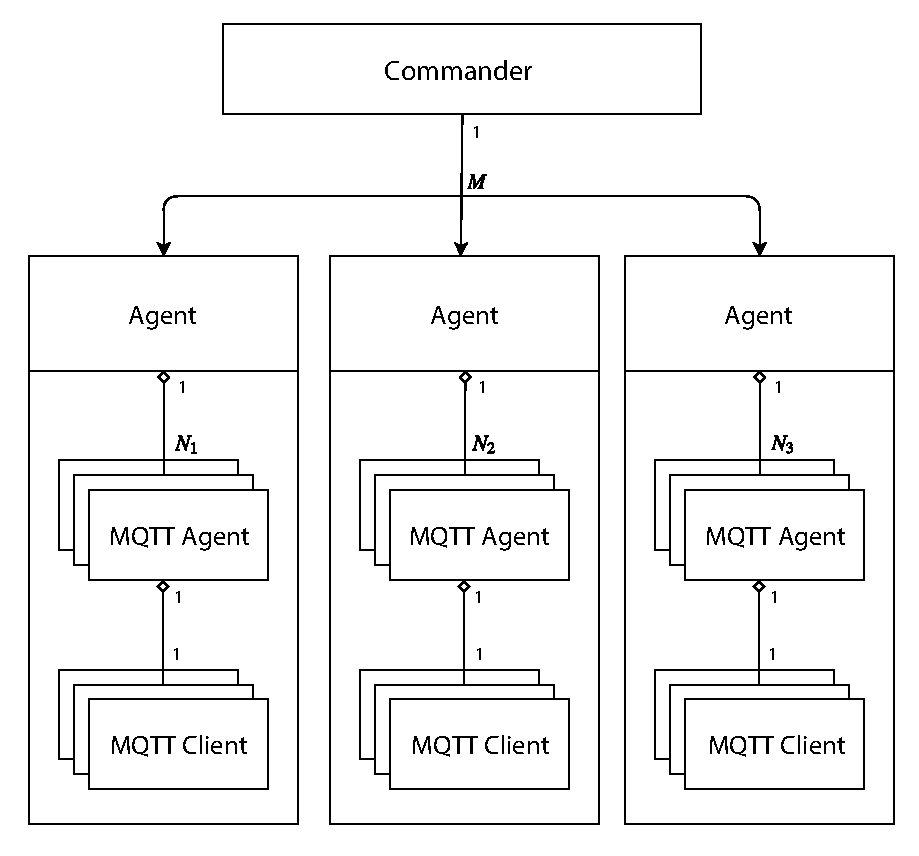
\includegraphics[scale=0.65]{Resources/PDF/Architecture}
	\caption{Varroa Distributed System Architecture}
	\label{pic:Architecture}
	\end{center}
\end{figure}
A Varroa Distributed System is composed of a Commander and multiple Agents.
The Commander and all Agents are executed in separate Varroa Instances.
Every Agent holds a number of MQTT Agents and each MQTT Agent manages one MQTT Client.
\newpage

\section{Commander}
\begin{figure}[h]
	\begin{center}
	\includegraphics[scale=1]{Resources/PDF/CommanderStates}
	\caption{Commander States}
	\label{pic:CommanderStates}
	\end{center}
\end{figure}

\section{Chunk Concept}
\subsection{Definition}
A chunk is a work package of the scenario execution designed to be distributed from the Commander to its Agents.
It is then handled by the Agent it is distributed to.
The Agent now creates or uses existing MQTT Agents to execute the Chunk.
It contains:
\begin{itemize}
	\item \textbf{clientCountInChunk}: the maximum amount of clients a chunk can represent.
	\item \textbf{clientOffset}: starting index of the clients contained in the chunk.
	\item \textbf{clientGroupId}: 
	\item \textbf{clientGroupInformation}: contains information concerning the Client Group and MQTT-specific properties.
	\item \textbf{stageDuration}: the duration of the stage this chunk belongs to.
	\item \textbf{lifecycleRate}: the rate at which the contained commands are executed.
	\item \textbf{commands}: a list of commands that are executed by the clients in the chunk.
\end{itemize}
%Due to the distributed nature of Varroa it was necessary to be able to spread the information contained in the scenario.
%To secure a deterministic distribution of a scenario's data the chunks had to be evenly spread across the initialized Agents.

\section{Chunk Distribution}
To secure a deterministic execution of a scenario the every chunk needs to be distributed to the same Agent in every execution of the scenario.
To ensure this determinism a mechanism was introduced combining a round-robin selection of chunks with a handshake mechanism of the agents.
\begin{figure}[h]
	\begin{center}
	\includegraphics[scale=1]{Resources/PDF/ChunkDistribution}
	\caption{Distribution of a Chunk}
	\label{pic:ChunkDistribution}
	\end{center}
\end{figure}

\section{Chunk Handshake}
\begin{figure}[h]
	\begin{center}
	\includegraphics[scale=1]{Resources/PDF/ChunkAcceptedHandshake}
	\caption{Chunk Handshake with Accept}
	\label{pic:ChunkAcceptedHandshake}
	\end{center}
\end{figure}

\begin{figure}[h]
	\begin{center}
	\includegraphics[scale=1]{Resources/PDF/ChunkRejectHandshake}
	\caption{Chunk Handshake with Reject}
	\label{pic:ChunkRejectHandshake}
	\end{center}
\end{figure}
\chapter{Reporting}\label{sec:Reporting}
\begin{lstlisting}[caption={Excerpt from a reporting output}, captionpos=b, label={lst:ReportingOutput}, language=]
--------------- Command Report ---------------
LifeCycle{lifeCycleId=waiters-1, clientGroupId=cg-1, clientCount=1}
Connect{brokerAddress=broker.hivemq.com:1883}={
	durationSampler=[count=1, mean=144ms, stdDev=0ns, min=144ms, max=144ms],
	latenessSampler=[-], failedCount=0}
Subscribe{subscription=[subscriptionId=subscription-1]}={
	durationSampler=[count=1, mean=26ms, stdDev=0ns, min=26ms, max=26ms],
	latenessSampler=[-], failedCount=0}
---------------- End  Report -----------------
\end{lstlisting}

Reporting is a core concept of Varroa.
Its purpose is to determine the results of a Varroa test and output them in a verifiable document.
For that reason there are entities that observe the parts of Varroa that execute the Scenario.
These exist on different hierarchy levels as later explained in \ref{sec:ReportingArchitecture}.
The reports are output in a PDF file and on the Commander's console output.
For the later an example is given in figure \ref{lst:ReportingOutput}.

\section{Command Report}
\begin{lstlisting}[caption={Example for a Command Report}, captionpos=b, label={lst:CommandReport}, language=]
--------------- Command Report ---------------
Publish{[...]}
For{times=5}={[...]}
---------------- End  Report -----------------
\end{lstlisting}
The Command Report contains aggregated metrics of every Command.
They are output in the order in which the Commands were defined in the Scenario.
With the exception of nested Commands, where the metrics of the inner Commands is output before those of the outer Command.
An example is given in figure \ref{lst:CommandReport}

\section{Action Report}
\begin{lstlisting}[caption={Excerpt from Action Report}, captionpos=b, label={lst:ActionReport}, language=]
--------------- Action Report ---------------
Publish{[...]}
Publish{[...]}
Publish{[...]}
Publish{[...]}
Publish{[...]}
For{times=5}={[...]}
---------------- End  Report -----------------
\end{lstlisting}
The Action Report allows for a finer analysis than the Report.
This is due to the fact that the Action Report does not aggregate the metrics of nested Commands like the For Command.
Instead it outputs all iterations contained in the For Command separately.
This difference becomes clear when comparing figure \ref{lst:CommandReport} and \ref{lst:ActionReport}.

\section{Reporting Architecture}\label{sec:ReportingArchitecture}
\begin{figure}[H]
	\begin{center}
		\includegraphics[scale=0.75]{Resources/PDF/ReportingArchitecture}
		\caption{Reporting Architecture}
		\label{fig:ReportingArchitecture}
	\end{center}
\end{figure}
The reporting architecture is organized in strong accordance to Varroas hierarchy.
The data flow of the report happens bottom up from the Agents to the Commander.
The reported data is recorded at the lowest level of the hierarchy namely the \emph{MqttAgentTracer} which tracks its MQTT Agents Actions.
Subsequently the \emph{AgentAggregator} receives this data and aggregates it before passing the result to the Commander.
The Commander aggregator collects the received data and then aggregates the information of all Agents and compiles it into the report.
Figure \ref{fig:ReportingArchitecture} visualizes the relationships between the components explained above.

\section{Metrics}
\subsection{Duration Sampler}
The duration Sampler gives metrics based on the duration of the executed Actions:
\begin{itemize}
	\item \textbf{count:} the amount of executed Actions.
	\item \textbf{mean:} the mean duration of the executed Actions.
	\item \textbf{stdDev:} the standard deviation of the duration of the executed Actions.
	\item \textbf{min:} the minimum duration of the executed Actions.
	\item \textbf{max:} the maximum duration of the executed Actions.
\end{itemize}
\subsection{Lateness Sampler}
The Duration Sampler reports metrics based on the lateness of expected durations of the executed Actions:
\begin{itemize}
	\item \textbf{count:} the amount of Actions whose durations exceeded the expected duration.
	\item \textbf{mean:} the mean lateness value of the actions.
	\item \textbf{stdDev:} the standard deviation of the executed Actions lateness.
	\item \textbf{min:} the minimum lateness of the executed Actions.
	\item \textbf{max:} the maximum lateness of the executed Actions.
\end{itemize}

\subsection{Failed Count}
The failed count indicates how many of the Actions are executed unsuccessfully.




\chapter{Requirements}
The following sections list the requirements and their respective priorities.
In addition, it is indicated whether and how they are currently implemented.

\section{Non-Functional Requirements}

\subsection{Transparency (Must Have High)}\label{sec:Transparency}
\emph{Varroa has to be comprehensible for the user.}

This requirement is fulfilled.
Varroa implements expressive logging with configurable levels and outputs.
This enables rich insight in the execution process of a Varroa test.

\subsection{10.000.000 MQTT Clients (Must Have High)} 
\emph{Varroa has to be able to generate a large amount of clients.}

The fulfilment of this requirement is not verified yet.

\subsection{Scalability (Must Have)} 
\emph{Varroa should scale vertically with relatively low scaling costs.}

This requirement is fulfilled.
To do so Varroa is organised as a distributed System and can easily be extended with new instances running as Varroa Agents.

\subsection{Determinism (Must Have)} 
\emph{Varroa has to work in deterministic ways, meaning it should produce the same result for a Scenario every time.}

This requirement is fulfilled.
To ensure this determinism several measures are taken in the distribution and execution of a Scenario (see chapter \ref{sec:Architecture}).

\subsection{Distributed (Must Have Low)} 
\emph{Varroa is a distributed System.}

This requirement is fulfilled.
Varroa is organized as a distributed System, it is composed of a Commander and multiple Agents that can run on different machines. 
 
\subsection{Usabillity (Very Important)} 
\emph{Varroa has to be easily usable.}

This requirement is fulfilled.
The user can easily define custom Scenarios as XML files and execute them (see chapter \ref{sec:ScenarioConcept} and \ref{sec:Execution}).

\subsection{Code Quality (Important)} 
\emph{Varroa's code quality should be very high.}

This requirement is fulfilled.
To ensure high code quality several measures are taken.
For example the consequent use of nullability annotiations and a broad test code coverage.
Also before new code could be added to the master branch it was reviewed by another team member.

\subsection{Stability (Important)} 
\emph{Varroa has to run in a stable manner.}

This requirement is fulfilled.
By the use of integration tests and general unit tests stability is ensured.

\subsection{Resource efficiency (Important)} 
\emph{Varroa has to use the available computation and memory resources efficiently.}
%TODO how was this verified.

\subsection{User / Developer Guide (Somewhat Important)} 
\emph{Varroa needs a User / Developer Guide.}

This requirement is fulfilled. This documentation educates the user on defining a custom scenario and after that executing it on his Varroa Distributed System (\ref{sec:ScenarioConcept} and \ref{sec:Execution}).

\subsection{Automation capacity (Somewhat Important)} 
\emph{Varroa should be automatable.}

%TODO Docker.
%TODO is this fulfilled? 

\subsection{User Interface}
\emph{Varroa should have a well designed user interface with high usability.}

This requirement is fulfilled.
The user can interact with Varroa using a command line interface.

\subsection{Multi Platform Support (Nice To Have)}
\emph{Varroa should run on multiple platforms.}

This requirement is fulfilled.
Due to the utilisation of Docker, Varroa can run on several platforms (see chapter \ref{sec:Execution}).

\section{Functional Requirements}
The following sections list the non-functional requirements and their respective priorities.

\subsection{Scenarios (Must Have High)}
\emph{Varroa must be able to execute user defined MQTT Scenarios.}

This requirement is fulfilled.
Varroa has the ability to parse and execute Scenarios, according to the concept explained in chapter \ref{sec:ScenarioConcept}.

\subsection{MQTT Specification Confirmity (Must Have High)}
\emph{Varroa must conform to the MQTT specification.}

This requirement is fulfilled.
Varroa uses the HiveMQ MQTT Client library for its MQTT actions.
The library ensures specification conformity in both MQTT version 3 and MQTT version 5.

\subsection{All Transports (Must Have)}
\emph{Varroa has to support all transports that are possible in MQTT.}

This requirement is not fulfilled.
Currently Varroa does not support websockets.

\subsection{Reports (Must Have)}
\emph{Varroa has to report the findings of the testing process.}

This requirement is fulfilled.
Varroa supports reporting findings of tests (see \ref{sec:Reporting})

\subsection{User Feedback (Must Have Low)}
\emph{Varroa has to give user feedback during runtime.}

This requirement is fulfilled (see \ref{sec:Transparency}).

\subsection{Documentation (Very Important)}
\emph{Varroa has to be documented. }

This requirement is fulfilled.
This document contains a user guide and briefly explains the architecture and inner workings of Varroa.

\subsection{Metrics (Very Important)}
\emph{Varroa has to record and expose internal metrics.}

This requirement is not fulfilled.

\subsection{Deployment Convenience (Important)}
\emph{Varroa must be easily deployable.}

This requirement is fulfilled. Due to the use of Docker Varroa Instances can be easily started and so a Varroa Distributed System can be orchestrated without much configuration (see chapter \ref{sec:Execution}).

\subsection{Topology Change (Less important)}
\emph{Varroa must be able to simulate changes to the network topology.}

This requirement is not fulfilled.
It is not possible to simulate network level behaviour of the clients in the current version.

\subsection{Simple and Expert Mode (Somewhat Important}
\emph{Varroa has to have two user modes.
One for experienced users and one for unexperienced users.}

This requirement is not fulfilled.
Since Varroa does not have a graphical user interface in this version.
Simple and Expert modes are not implemented.


\subsection{Notifications (Nice To Have)}
\emph{Varroa must notitfy the user about the testing process by Email.}

This requirement is not fulfilled in the current version.





















% Abbildungsverzeichnis generieren.
\clearpage
\addcontentsline{toc}{chapter}{\listfigurename}
\listoffigures

% Tabellenverzeichnis generieren.
\clearpage
\addcontentsline{toc}{chapter}{\listtablename}
\listoftables

% Listingverzeichnis generieren.
\clearpage
\renewcommand{\lstlistlistingname}{Listingverzeichnis}
\addcontentsline{toc}{chapter}{\lstlistlistingname}
\lstlistoflistings

\end{document}
